% $Id: chapter3.tex 1790 2010-09-28 16:46:40Z jabriffa $

\chapter{Technical Review}

This chapter will go in depth about technical side of the project. It will start off with the dataset that being used. Then, it will discuss the resources that will be used and where the code and the models will be from. After then, will walk through each of the models that are implemented and the usage of libraries and methods.

\section{Dataset}
The dataset that is used to train and test is from \textit{"Emotion Dataset for Emotion Recognition Tasks"} \cite{Pandey_2021} from Kaggle which is based from \textit{"CARER: Contextualized Affect Representations for Emotion Recognition"} \cite{saravia-etal-2018-carer} paper. It is an English Twitter message dataset, and it has 6 labels: sadness (0), joy (1), love (2), anger (3), fear (4) and surprise (5). It is for single-label emotion classification task, and it is already separated into train, test and validation dataset. The dataset is preprocessed by removing any special characters and punctuations, and upper-cased are all lower-cased. Removing stop-word could affect the model performance as every word has to be contextualized.

\textbf{An example of 'train' dataset:} 

\emph{"label": 0,}

\textit{"text": "im feeling quite sad and sorry for myself but ill snap out of it soon" }
\begin{figure}[ht]
    \centerline{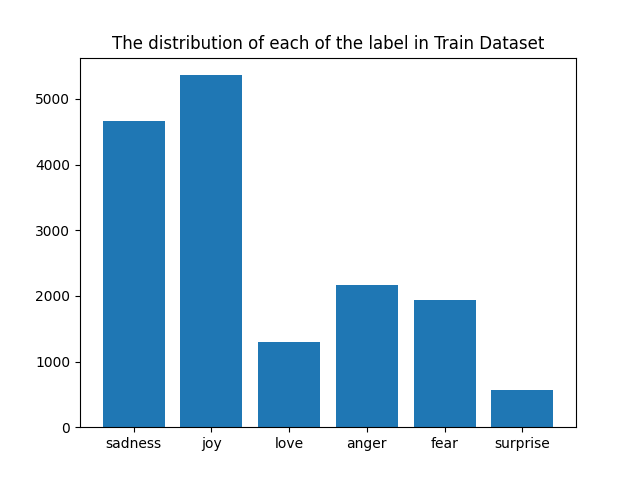
\includegraphics[scale=0.5]{Figures/dataset_distribution.png}}
    \caption{The graph for the distribution of each label in Train dataset}
    \label{fig:dataset}
\end{figure}

The distribution of each label for train dataset is not equal, the most being joy and the least being surprise. The Figure[\ref{fig:dataset}] will show the distribution of train dataset. 

\section{Methods}

This section will dive deeper into each pre-trained model, and how it is implemented, what libraries have been used and why. The 4 pre-trained transformer models that are implemented for this research are as mentioned in literature review which are miniLM, Llama2, RoBERTa and GPT-2.

\begin{figure}[ht]
    \centerline{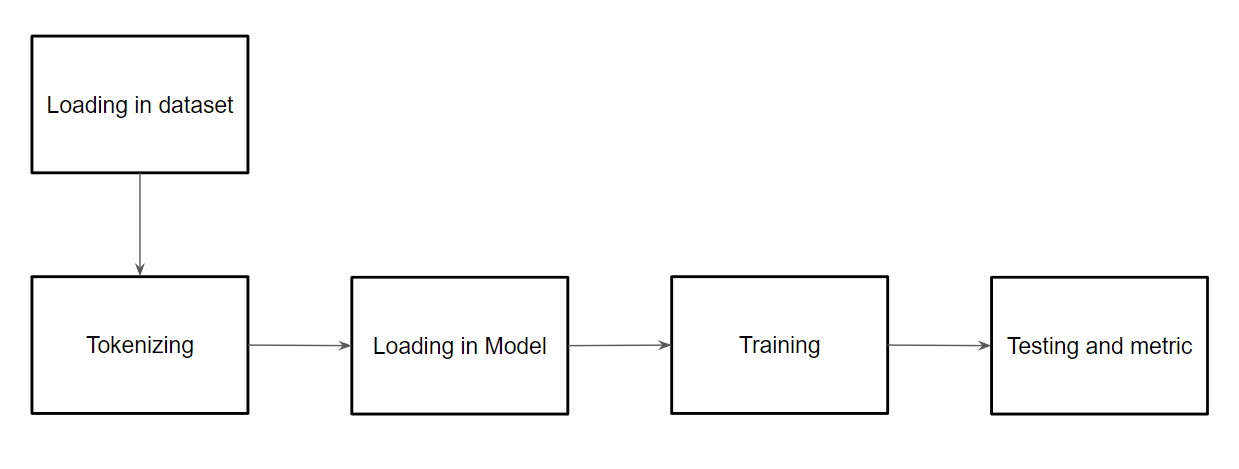
\includegraphics[scale=0.45]{Figures/problem_pipeline.png}}
    \caption{A pipeline of the overall flow of implementation}
    \label{fig:pipeline}
\end{figure}

The Figure[\ref{fig:pipeline}] shows the overall implementation of each model. The code for all the model will be followed roughly as the figure portrays and will be sectioned as such: Import libraries, Dataset, Model, Training and Testing/Evaluation. The implemented models will be run as Notebooks on either Google Colab or locally (in Vscode) depending on how big the model is.

The main benefit of using notebooks for the implementation is ability to break sections of code into blocks of code or 'cells' to make it easier to see and follow through. It also makes sectioned code easier to test and check for errors. For example, if the variables or code need to be checked to ensure their functionalities, or to check the features of datasets, cells can be added to verify and deleted after. Another benefit is that the cells can be 'markdown cells' which allow the code to section up with titles and paragraphs overviewing each section, allowing anyone to understand the code quicker.

The pretrained models that I used for the implementation are all from huggingface. Huggingface is a substantial platform for an AI community. It's also accommodating for any new keen learner with their work through videos and documents. It also provides many tools such as different models, datasets, accessibilities to any Ai applications made by the community, documents for specific libraries and methods, solutions and finally an ability to communicate or ask about any Ai related queries with other members in the community.

\subsection{Main libraries}
The following are the libraries used throughout all the models that are implemented, and the brief descriptions of their use and what they provide:

\textbf{Torch:} an essential python library which allows machine learning algorithms to run faster than if they were written in normal python. It also supports 'Cuda' to run models on the GPU.

\textbf{Datasets:} a library that provides easy access for loading in datasets from huggingface as well as your own datasets.

\textbf{Transformers:} give an ability to load in all the transformer models, provide tools such as Trainer, TrainingArguments and so on and pipeline from the huggingface.

\textbf{Pandas:} used for reformatting and organizing the datasets without actual changes to the datasets.

\textbf{TQDM:} displays progress of the model training and testing.


\subsection{MiniLM}
The English pre-trained model checkpoint that is loaded from huggingface is \textit{'microsoft/MiniLM-L12-H384-uncased'}. It is the uncased 12-layer model with 384 hidden size distilled from an in-house pre-trained UniLM v2 model (it is not available for public) in BERT-base, 33 million parameters, and it is 2.7 times faster than BERT-Base \cite{patrickvonplaten}.


\subsection{Llama2}
  
\subsection{RoBERTa}

\subsection{GPT-2}


\section{Metrics}

\textbf{Sklearn.metrics:} used for generating metrics such as accuracy, confusion matrix and so on for the evaluation.
